\documentclass{article}
\usepackage{amsmath}
\usepackage{graphicx}
\usepackage{hyperref}
\usepackage{listings}
\begin{document}
\title{Applied Large Language Models}
\maketitle
\section{Deployment \& Inference
Optimization}\label{deployment-inference-optimization}

\begin{itemize}
\item
  Quantization -- int8/bfloat16 inference.
\item
  Low-rank adaptation -- LoRA for efficient fine-tuning and inference.
\item
  Pruning -- structured vs unstructured.
\item
  Knowledge distillation -- student-teacher training.
\item
  Batching strategies for inference -- microbatching, dynamic batching
  for latency-sensitive endpoints
\item
  Early exit models -- stopping inference when confident.
\end{itemize}

\subsection{How Inference Works}\label{how-inference-works}

how LLMs actually generate text. The process can be broken down into two
main phases: prefill and decode. These phases work together like an
assembly line, each playing a crucial role in producing coherent text.

\textbf{Prefill phase} is like the preparation stage in cooking - it's
where all the initial ingredients are processed and made ready.

\begin{itemize}
\item
  Tokenization: Converting the input text into tokens (think of these as
  the basic building blocks the model understands)
\item
  Embedding Conversion: Transforming these tokens into numerical
  representations that capture their meaning
\item
  Initial Processing: Running these embeddings through the model's
  neural networks to create a rich understanding of the context
\end{itemize}

This phase is computationally intensive because it needs to process all
input tokens at once.

\textbf{The Decode Phase.} The model generates one token at a time in
what we call an autoregressive process (where each new token depends on
all previous tokens).

\begin{itemize}
\item
  Attention Computation: Looking back at all previous tokens to
  understand context
\item
  Probability Calculation: Determining the likelihood of each possible
  next token
\item
  Token Selection: Choosing the next token based on these probabilities
\item
  Continuation Check: Deciding whether to continue or stop generation
\end{itemize}

This phase is memory-intensive because the model needs to keep track of
all previously generated tokens and their relationships.


\textbf{Managing Repetition} One common challenge with LLMs is their
tendency to repeat themselves - much like a speaker who keeps returning
to the same points. To address this, we use two types of penalties:

\begin{itemize}
\item
  Presence Penalty: A fixed penalty applied to any token that has
  appeared before, regardless of how often. This helps prevent the model
  from reusing the same words.
\item
  Frequency Penalty: A scaling penalty that increases based on how often
  a token has been used. The more a word appears, the less likely it is
  to be chosen again.
\end{itemize}

These penalties are applied early in the token selection process,
adjusting the raw probabilities before other sampling strategies are
applied. Think of them as gentle nudges encouraging the model to explore
new vocabulary.


\textbf{Temperature Control}: Like a creativity dial - higher settings
(\textgreater1.0) make choices more random and creative, lower settings
(\textless1.0) make them more focused and deterministic. This is done by
scaling the logits (raw scores) before applying the softmax function to
get probabilities: 
\[
P(x_i) = \frac{e^{(p_i / \tau)}}{\sum_{j} e^{(p_j / \tau)}}
\],

where \(p_i\) is the logit for token \(i\) and \(\tau\) is the
temperature. A higher temperature flattens the distribution, making less
likely tokens more probable, while a lower temperature sharpens it,
favoring the most likely tokens.\\

\textbf{Filtering Strategies} 
\begin{itemize}
\item Top-p (Nucleus) Sampling: Instead of considering all possible words, we only look at the most likely ones that add up to our chosen probability threshold (e.g., top 90\%)
\item Top-k Filtering: An alternative approach where we only consider the \(k\) most likely next words
\end{itemize}

\textbf{Controlling Generation Length} 

\begin{itemize}
\item Token Limits: Setting minimum and maximum token counts
\item Stop Sequences: Defining specific patterns that signal the end of generation
\item End-of-Sequence Detection: Letting the model naturally conclude its response
\end{itemize}

For example, if we want to generate a single paragraph, we might set a
maximum of 100 tokens and use ``\\n\\n'' as a stop sequence.

\subsubsection{Beam Search}\label{beam-search}

\begin{figure}
\centering
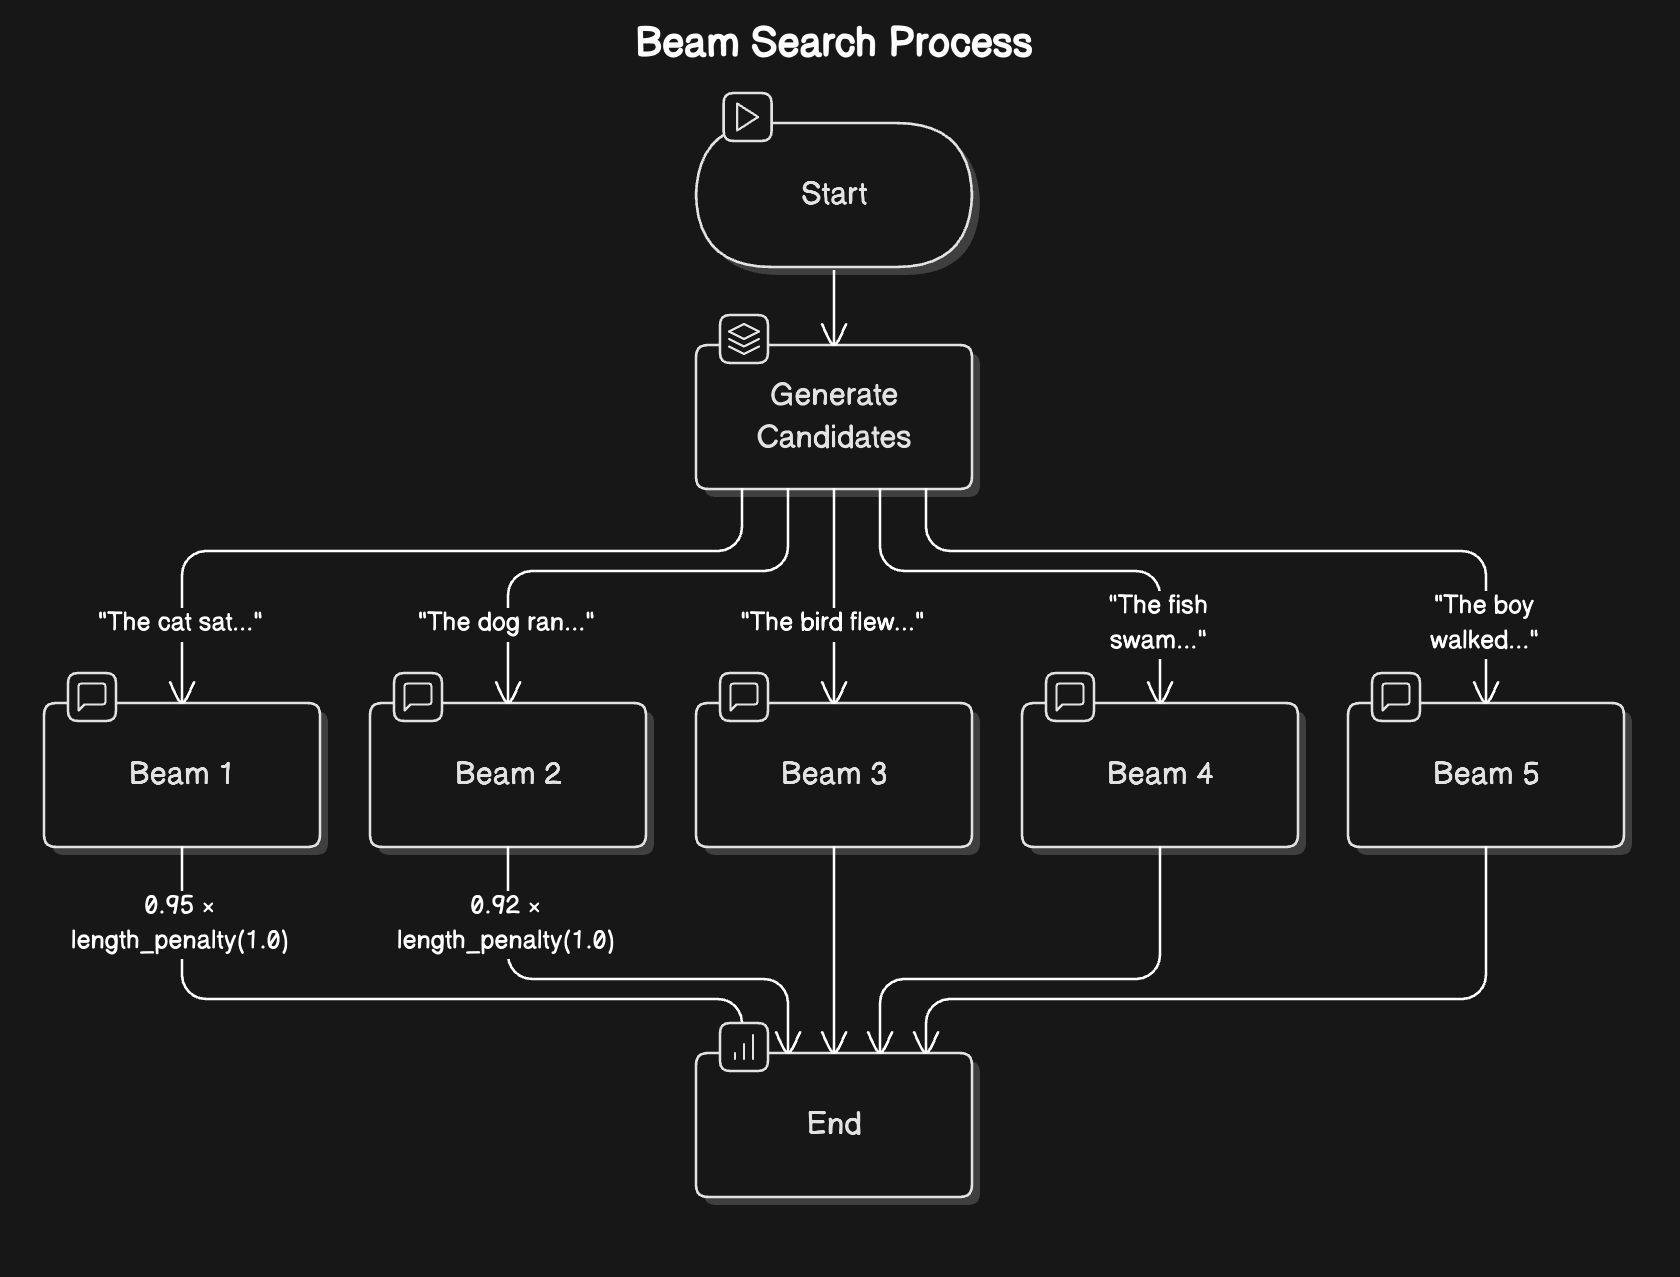
\includegraphics[width=0.75\textwidth,alt={Beam Search Illustration}]{./images/beam-search.png}
\caption{Beam Search Illustration}
\end{figure}

While the strategies we've discussed so far make decisions one token at
a time, beam search takes a more holistic approach. Instead of
committing to a single choice at each step, it explores multiple
possible paths simultaneously - like a chess player thinking several
moves ahead. 

\begin{enumerate}
\item At each step, maintain multiple candidate sequences(typically 5-10) 
\item For each candidate, compute probabilities for the next token 
\item Keep only the most promising combinations of sequences and next tokens 
\item Continue this process until reaching the desired length or stop condition 
\item Select the sequence with the highest overall probability
\end{enumerate}

\subsection{Tools}\label{tools}

\begin{itemize}
\item \href{https://huggingface.co/docs/bitsandbytes/main/en/index}{bitsandbytes}
\item \href{https://triton-lang.org/}{Triton}
\item \href{https://developer.nvidia.com/tensorrt}{TensorRT}
\end{itemize}

\subsubsection{FlashAttention and FlashAttention2}\label{flashattention-and-flashattention2}

FlashAttention is an optimized attention mechanism designed to improve
the efficiency of transformer models during inference and training.
Traditional attention mechanisms can be memory-intensive and slow,
especially for long sequences, due to the quadratic complexity of
computing attention scores. FlashAttention addresses these challenges by
implementing a more memory-efficient algorithm that reduces the amount
of data that needs to be stored in memory at any given time.

FlashAttention achieves its efficiency through several key techniques:

\begin{enumerate}
\item Memory-Efficient Computation: It computes attention scores in a way that minimizes memory usage, allowing for larger batch sizes and longer sequences without running out of memory. 
\item Kernel Fusion: By combining multiple operations into a single kernel, FlashAttention reduces the overhead associated with launching multiple GPU kernels, leading to faster execution. 
\item Reduced Precision: FlashAttention can leverage lower-precision arithmetic (e.g., FP16) to speed up computations while maintaining acceptable accuracy.
\end{enumerate}

\begin{figure}
\centering
% 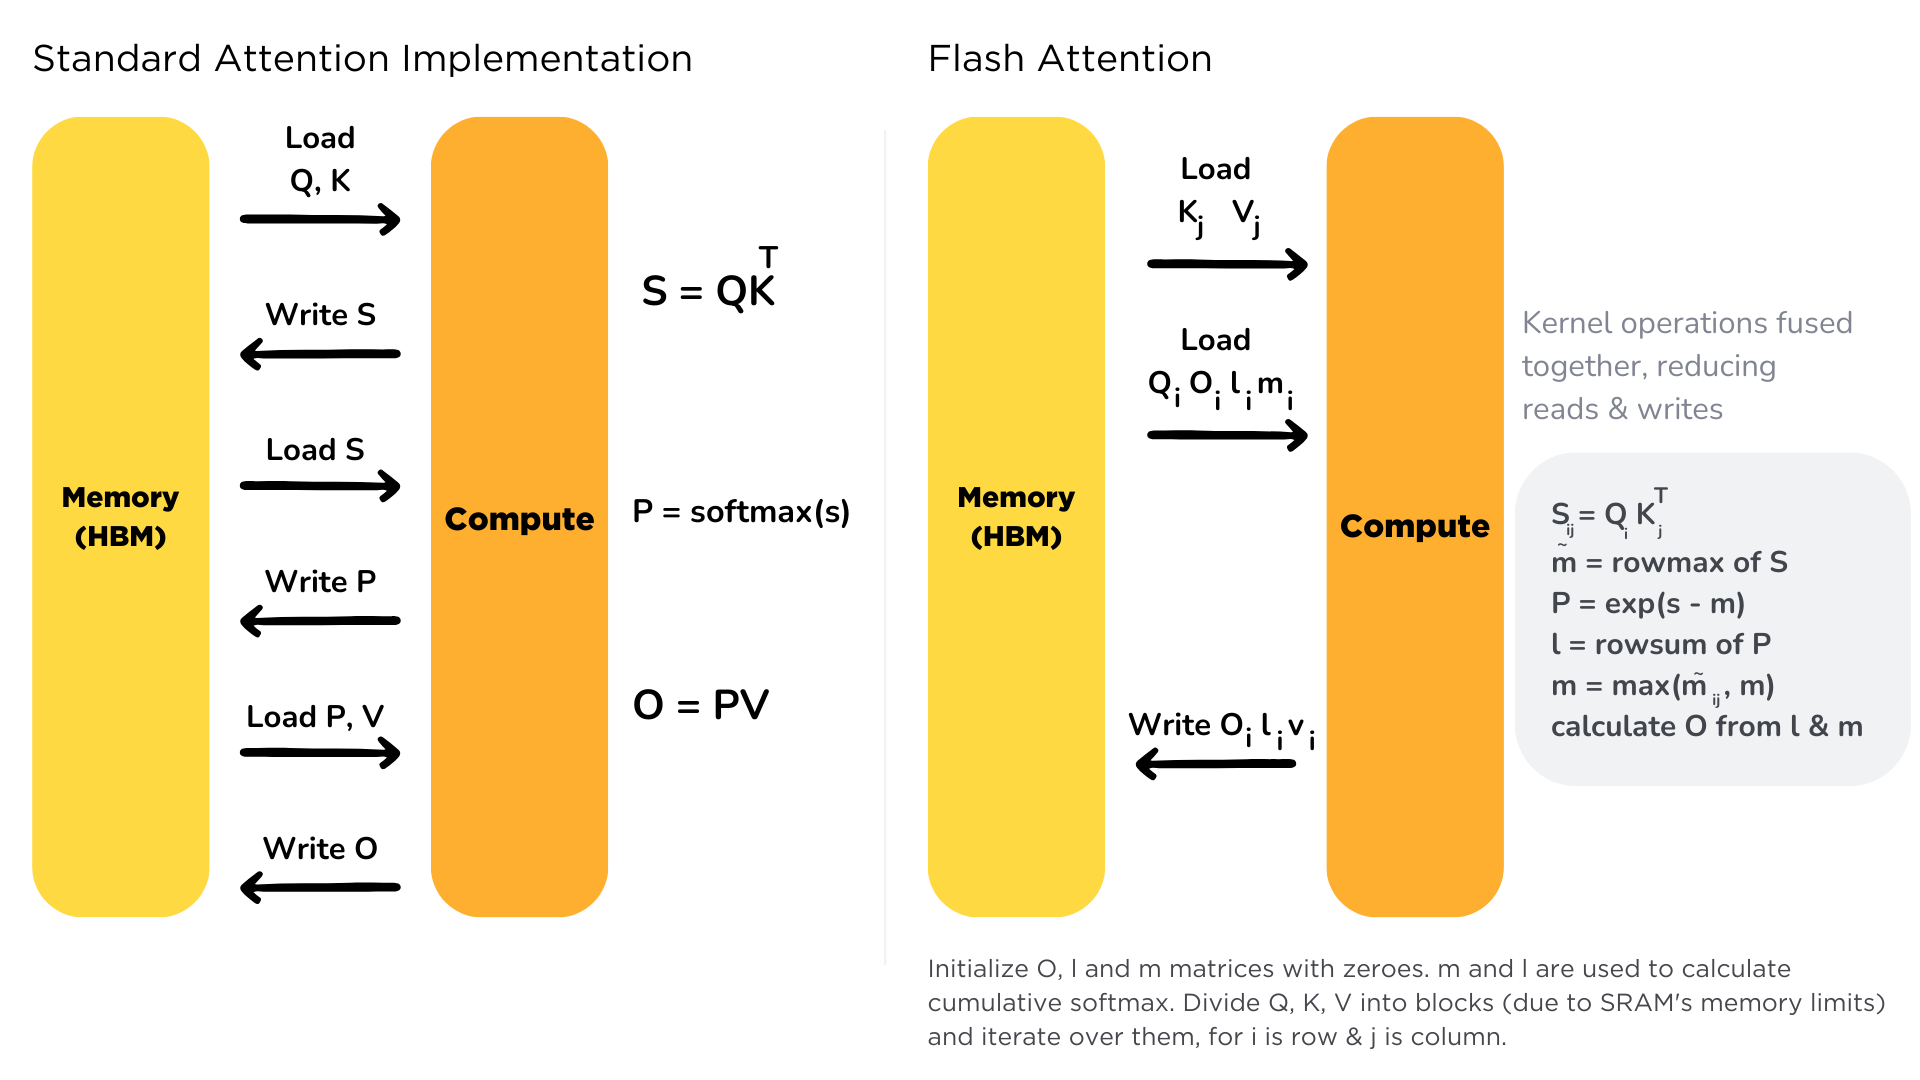
\includegraphics[keepaspectratio,alt={Flash Attention Diagram}]{./images/flash-attn.png}
% set smaller aspect ratio
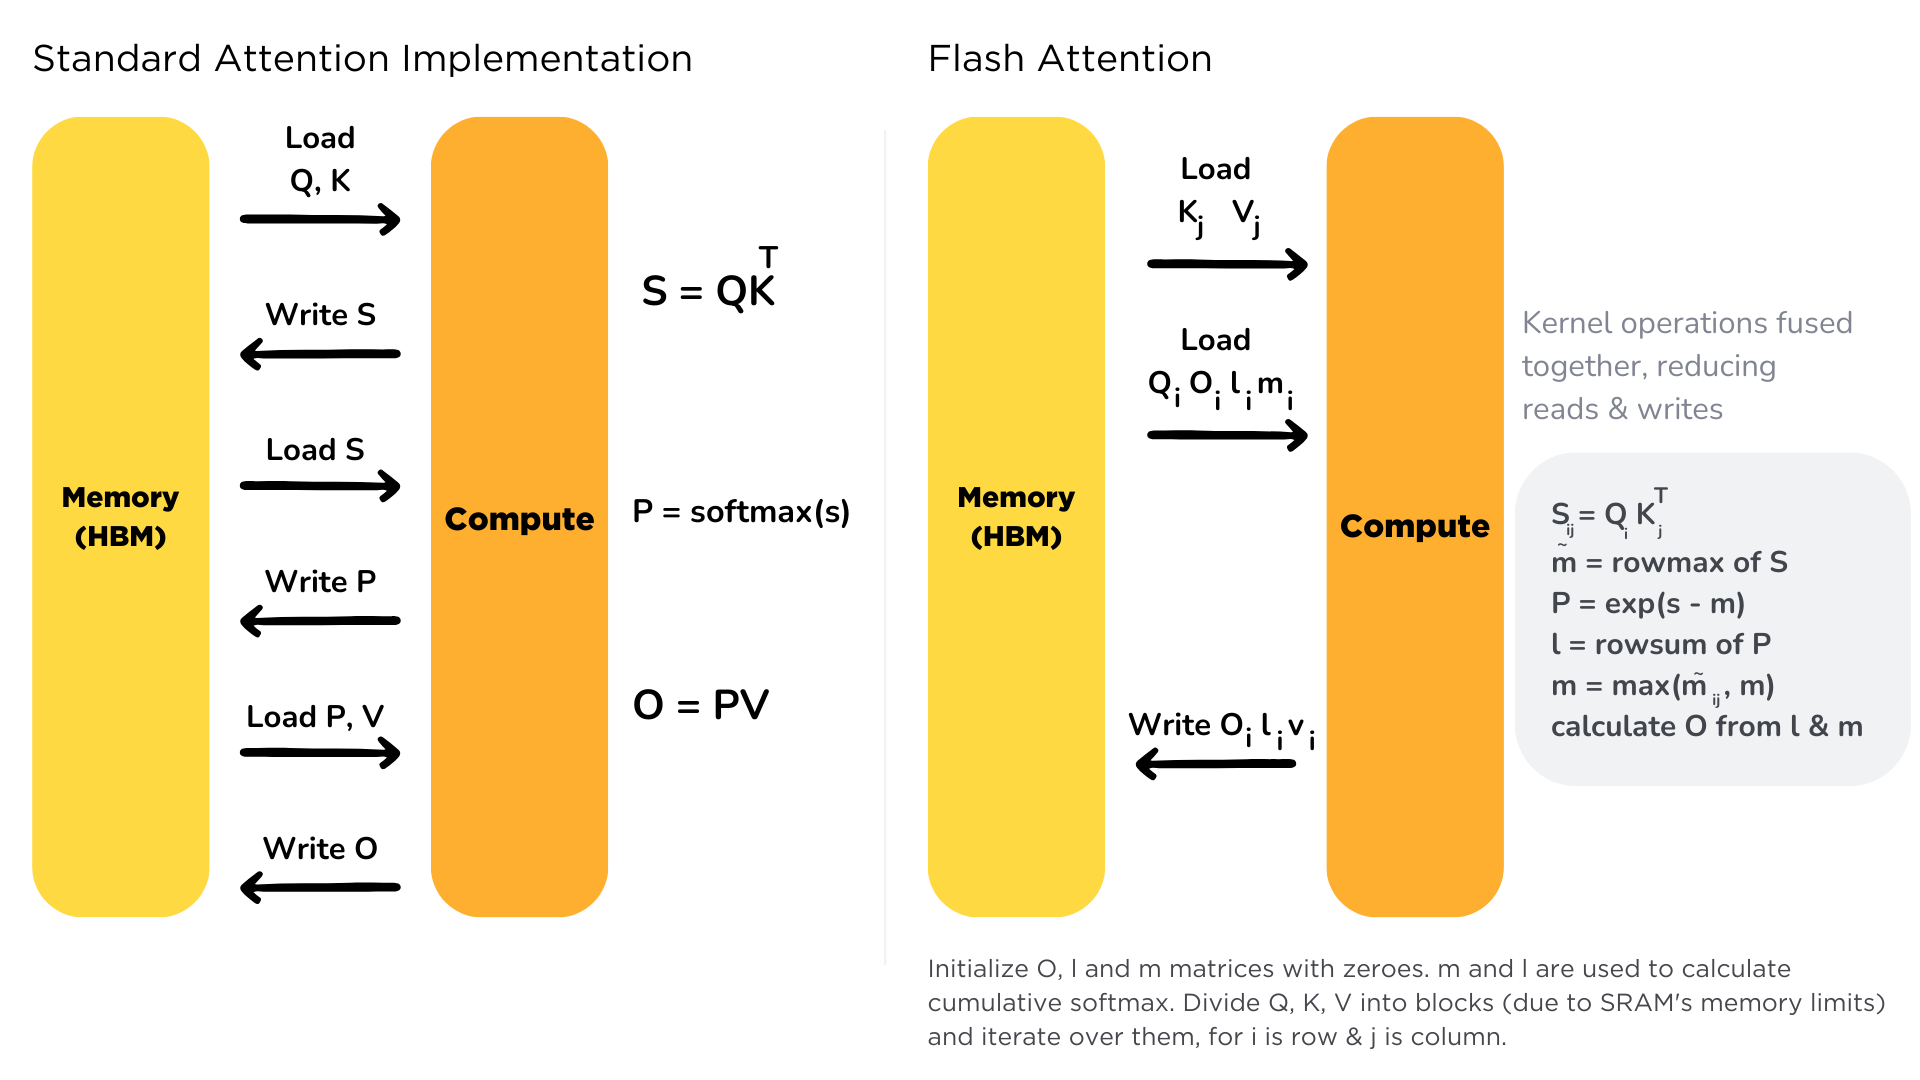
\includegraphics[width=0.75\textwidth,alt={Flash Attention Diagram}]{./images/flash-attn.png}
\caption{Flash Attention Diagram}
\end{figure}

FlashAttention2 builds upon the original FlashAttention by further optimizing the attention computation process. It introduces additional improvements such as better handling of variable-length sequences and enhanced support for different hardware architectures.

FlashAttention2 also incorporates more advanced techniques for reducing memory bandwidth usage, which is often a bottleneck in high-performance computing.

\textbf{Text Generation Inference (TGI)} is designed to be stable and
predictable in production, using fixed sequence lengths to keep memory
usage consistent. TGI manages memory using Flash Attention 2 and
continuous batching techniques. This means it can process attention
calculations very efficiently and keep the GPU busy by constantly
feeding it work. The system can move parts of the model between CPU and
GPU when needed, which helps handle larger models.

\subsubsection{llama.cpp}\label{llama.cpp}

llama.cpp is a highly optimized C/C++ implementation originally designed
for running LLaMA models on consumer hardware. It focuses on CPU
efficiency with optional GPU acceleration and is ideal for
resource-constrained environments. llama.cpp uses quantization
techniques to reduce model size and memory requirements while
maintaining good performance. It implements optimized kernels for
various CPU architectures and supports basic KV cache management for
efficient token generation.

Quantization in llama.cpp reduces the precision of model weights from
32-bit or 16-bit floating point to lower precision formats like 8-bit
integers (INT8), 4-bit, or even lower. This significantly reduces memory
usage and improves inference speed with minimal quality loss.

Key quantization features in llama.cpp include:

\begin{itemize}
%\tightlist
\item
  Multiple Quantization Levels: Supports 8-bit, 4-bit, 3-bit, and even
  2-bit quantization
\end{itemize}

GGML/GGUF Format: Uses custom tensor formats optimized for quantized
inference

\begin{itemize}
\item
  Mixed Precision: Can apply different quantization levels to different
  parts of the model
\item
  Hardware-Specific Optimizations: Includes optimized code paths for
  various CPU architectures (AVX2, AVX-512, NEON)
\end{itemize}

This approach enables running billion-parameter models on consumer
hardware with limited memory, making it perfect for local deployments
and edge devices.

\subsubsection{vLLM}\label{vllm}

vLLM takes a different approach by using PagedAttention. Just like how a
computer manages its memory in pages, vLLM splits the model's memory
into smaller blocks. This clever system means it can handle
different-sized requests more flexibly and doesn't waste memory space.
It's particularly good at sharing memory between different requests and
reduces memory fragmentation, which makes the whole system more
efficient.

PagedAttention is a technique that addresses another critical bottleneck
in LLM inference: KV cache memory management. During text generation,
the model stores attention keys and values (KV cache) for each generated
token to reduce redundant computations. The KV cache can become
enormous, especially with long sequences or multiple concurrent
requests.

vLLM's key innovation lies in how it manages this cache:

\begin{enumerate}
\def\labelenumi{\arabic{enumi}.}
%\tightlist
\item
  Memory Paging: Instead of treating the KV cache as one large block,
  it's divided into fixed-size ``pages'' (similar to virtual memory in
  operating systems).
\item
  Non-contiguous Storage: Pages don't need to be stored contiguously in
  GPU memory, allowing for more flexible memory allocation.
\item
  Page Table Management: A page table tracks which pages belong to which
  sequence, enabling efficient lookup and access.
\item
  Memory Sharing: For operations like parallel sampling, pages storing
  the KV cache for the prompt can be shared across multiple sequences.
\end{enumerate}

The PagedAttention approach can lead to up to 24x higher throughput
compared to traditional methods, making it a game-changer for production
LLM deployments.

\subsubsection{ONNX / TorchScript export -- framework-agnostic
inference.}\label{onnx-torchscript-export-framework-agnostic-inference.}

Open Neural Network Exchange (ONNX) and TorchScript are two popular
formats for exporting machine learning models to enable
framework-agnostic inference.

\subsection{Measuring Inference
Efficiency}\label{measuring-inference-efficiency}

When evaluating the efficiency of LLM inference, consider the following
metrics: * Latency: The time it takes to generate a response, typically
measured in milliseconds. Lower latency is crucial for real-time
applications. * Throughput: The number of requests the model can handle
per second. Higher throughput indicates better efficiency, especially
for batch processing. * RTFx: Real-Time Factor (RTF) measures how
quickly a model generates text relative to real-time. An RTF of 1 means
the model generates text at the same speed as a human speaks, while an
RTF less than 1 indicates faster-than-real-time generation. * Resource
Utilization: Monitor CPU, GPU, and memory usage during inference.
Efficient models should maximize performance while minimizing resource
consumption. * Cost Efficiency: Calculate the cost per inference
request, factoring in cloud compute costs. More efficient models should
deliver lower costs for the same performance level. * Scalability:
Assess how well the model performs as the number of concurrent requests
increases. Efficient models should maintain performance under load. *
Energy Consumption: Measure the power usage during inference. Lower
energy consumption is beneficial for both cost savings and environmental
impact. * Time-to-First Token (TTFT): The time taken from receiving a
request to generating the first token. This is particularly important
for user-facing applications where responsiveness is key.

\subsection{KV Caching}\label{kv-caching}

\subsection{References}\label{references}

\begin{itemize}
\item
  https://huggingface.co/learn/llm-course/chapter1/8
\item
  https://magazine.sebastianraschka.com/p/coding-the-kv-cache-in-llms
\item
  https://docs.vllm.ai/en/latest/contributing/
\item
  https://huggingface.co/learn/llm-course/chapter2/8
\end{itemize}
\end{document}